\chapter{Tvorba aplikace}
\label{4-tvorba-aplikace}

\section{Vytvoření základní aplikace}

Aplikace, která byla vytvořena v projektu \zk{FGIS} nebyla vytvořena
správně, obsahovala zbytečně složitý a chybný kód. Začalo se tedy
od začátku. Nejprve byl vytvořen projekt příkazem {\tt django-admin 
startproject mysite}. V projektu následně byla vytvořena aplikace
pomocí {\tt python manage.py startapp}. Aplikace byla v
\emph{settings.py} přidána do INSTALLED\_APPS. Dále se
nastavilo připojení k databázi. V \emph{settings.py} se tedy v
DATABASES se změnil engine na MySQL, protože Django v základu
používá SQLite. Změnilo se ještě NAME, USER, PASSWORD, HOST A PORT,
protože databáze byla provozována na školním serveru
\emph{geo102.fsv.cvut.cz}. Po připojení se musel vygenerovat model databáze
příkazem inspectdb. Dále byla
provedena migrace, aby se v databázi vytvořily Django
tabulky. Posledním krokem bylo vytvoření superuživatele, který se bude
moci přihlásit do uživatelské i administrátorské aplikace. To bylo
realizováno příkazem {\tt python manage.py createsuperuser}.

Na stránce GitLab.com byl vytvořen nový repozitář, do kterého se celý
projekt přesunul a nadále v něm byl průběžně zálohován. Dále se tam
vytvářely tzv. \emph{issues}, kde se plánovaly nadcházející úkoly při
tvorbě aplikace.

\section{Tvorba aplikace v uživatelském prostředí}
Při vytváření uživatelské aplikace bylo postupováno dle příkladu v \cite{django-for-beginners}.
Prvním větším úkolem bylo vytvořit aplikaci, která bude zobrazovat
data a po přihlášení je bude moci uživatel také přidávat, mazat a
editovat. Nejprve se tedy do adresáře aplikace přidal soubor \emph{urls.py},
který se následně připojil k \emph{urls.py} v projektovém adresáři. Tento
způsob je výhodný při použití více aplikací, kdy si každá aplikace
uchovává své \zk{URL} adresy a projekt je tak přehlednější. Pokračovalo se
vytvořením pohledů založených na třídách, které se v Pythonu používají
pro nahrazení pohledů jako funkcí. Použity jsou základní pohledy jako
ListView pro zobrazení obsahu tabulky nebo CreateView pro uložení dat
do databáze. V aplikaci v soubory \emph{views.py} jsou tedy vytvořeny
třídy pohledů pro každou \zk{URL} adresu. Definice těchto tříd vypadá
následovně \emph{class “název třídy“(Listview):} dále se u třídy
definuje model, který se má zobrazit a template\_name neboli název
šablony, která se použije při zobrazení.

\begin{figure}[H] \centering
    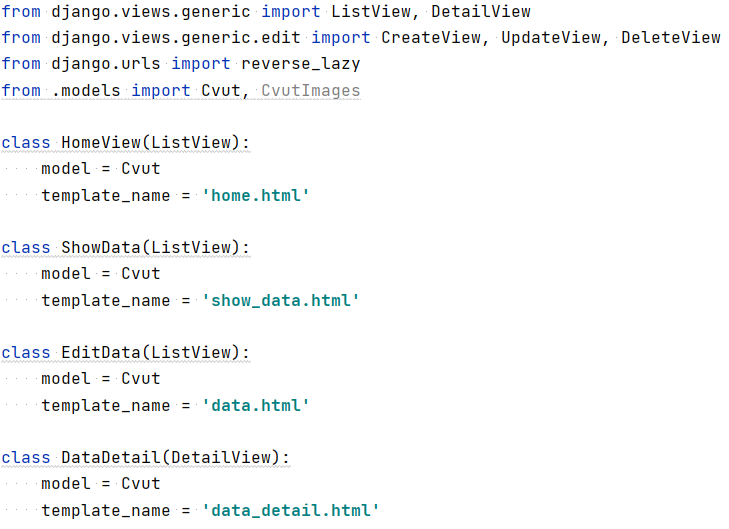
\includegraphics[width=350pt]{./pictures/6-nahled-views-aplikace.PNG}
    \caption[Náhled views.py a jeho tříd]{Náhled views.py a jeho tříd}
	\label{fig:Náhled views.py a jeho tříd}              
\end{figure}


V souboru \emph{urls.py} jsou propojeny \zk{URL} adresy, pohledy a \zk{HTML}
šablony, na které se odkazují. Do \emph{urls.py} musí být zároveň importovány
všechny použité pohledy. Dále je potřeba vložit cestu příkazem \emph{import path}. 
Poté se sestaví urlpatterns, což je seznam, který obsahuje jednotlivé
adresy. Ty jsou v něm uvedeny ve funkci path, která má dva povinné
argumenty, route a view a dva nepovinné, name a kwargs. Route uvádí
adresu, pod jakou se bude stránka načítat a view odkazuje na
importovaný pohled. Zde byla použita funkce \emph{as\_view()}, která
se používá, pokud je pohled typu třída. Jméno je uvedeno jako název
\zk{HTML} šablony.

\begin{figure}[H] \centering
    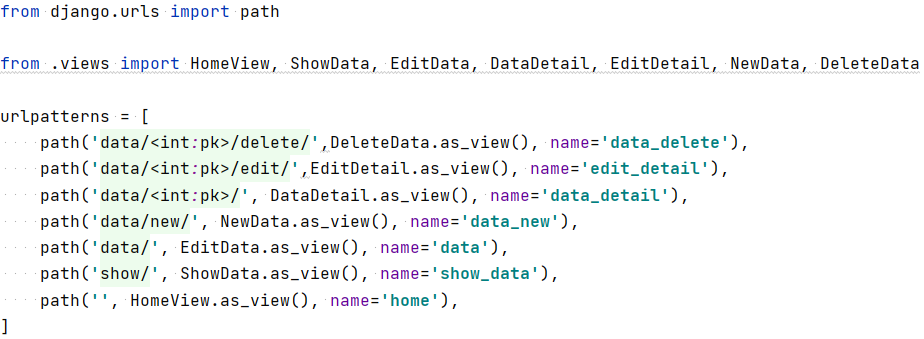
\includegraphics[width=450pt]{./pictures/7-urls-aplikace.PNG}
    \caption[Náhled urls.py v adresáři aplikaci]{Náhled urls.py v adresáři aplikaci}
	\label{fig:Náhled urls.py v adresáři aplikaci}              
\end{figure}

Pro vytvoření \zk{HTML} šablon se vytvořila složka \emph{templates}, kde
jsou uloženy jednotlivé \zk{HTML} soubory. Tato složka se v \emph{settings.py}
nastaví jako výchozí pro jejich zobrazení. Poté se už mohou vytvářet
jednotlivé šablony. Šablony jsou vždy vytvořeny s podmínkou \emph{if
  user.is\_authenticated}, tedy pokud je uživatel přihlášen, zobrazí
se mu na stránce možnosti data editovat, vytvářet a mazat. S tímto je
spojena ještě další změna v \emph{settings.py}, kde je přidáno
LOGIN\_REDIRECT\_URL = 'home' a LOGOUT\_REDIRECT\_URL
  = 'home' které uživatele po přihlášení a odhlášení přesměruje na
domovskou stránku. Ve složce \emph{templates} je ještě složka
\emph{registration}, kde je umístěn \emph{login.html}. \zk{HTML} soubory
zobrazují data v základní formě tabulek a nejsou graficky upravována
pomocí \zk{CSS} (Cascading Style Sheets).

\begin{figure}[H] \centering
    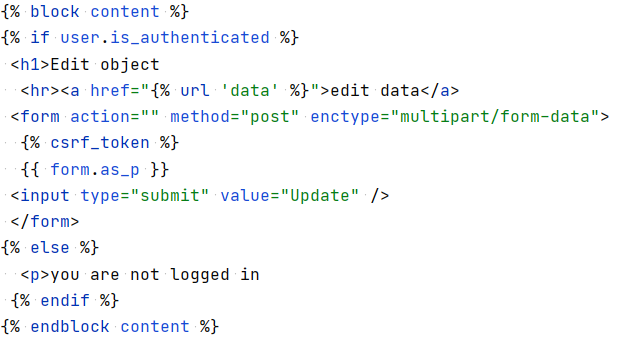
\includegraphics[width=350pt]{./pictures/8-edit-detail-html.PNG}
    \caption[Náhled HTML souboru edit detail]{Náhled HTML souboru edit detail}
	\label{fig:Náhled HTML souboru edit detail}
\end{figure}


\newpage

\section{Přidání obrázků}
\label{Přidání obrázků}

Dalším úkolem bylo vyřešit přidávání obrázků k jednotlivým
záznamům. Obrázky se neměly ukládat do databáze, ale do adresáře v
aplikaci. Databáze poté měla obsahovat cestu k těmto souborům. K tomu
byla vytvořena nová tabulka, který byla přes cizí klíč spojena s
tabulkou se záznamy. Tabulka byla vytvořena v modelu, a poté pomocí
migrací byla přenesena do databáze. Obsahuje tedy pole \zk{ID}, což je
primární klíč tabulky, Post, který je cizím klíčem k tabulce Cvut a
sloupec Image, do kterého se zaznamenává cesta k danému souboru viz \ref{fig:Struktura výběrové databáze}.
Pro zobrazení obrázků ještě musel být doinstalován přídavný modul Pillow.


\begin{figure}[H] \centering
    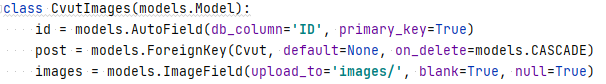
\includegraphics[width=430pt]{./pictures/9-db-cvutimages.PNG}
    \caption[Náhled tabulky CvutImages pro ukládání obrázků]{Náhled tabulky CvutImages pro ukládání obrázk}
	\label{fig:Náhled tabulky CvutImages pro ukládání obrázk}              
\end{figure}


V nastavení se dále určí kořenový adresář pro nahrávané soubory
MEDIA\_ROOT = os.path.join(BASE\_DIR, 'media') a
MEDIA\_URL = '/media/'.  A v poslední řadě se musí nastavit v
projektovém \emph{urls.py} media soubory, které Django samo neumí
zobrazovat. Zde se provede import settings a static a k urlpatterns se
připojí funkce static.

\begin{figure}[H] \centering
    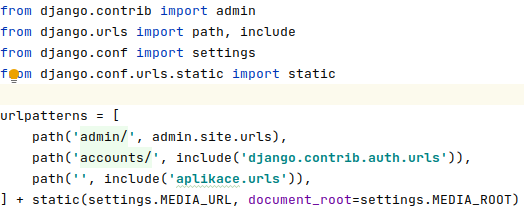
\includegraphics[width=380pt]{./pictures/10-media-urlspy.PNG}
    \caption[Náhled projektového urls.py]{Náhled projektového urls.py}
	\label{fig:Náhled projektového urls.py}              
\end{figure}

\newpage

\section{Statické soubory}

Pro řešení vizuální stránky webu jsou používány \zk{CSS} soubory. Ve složce
aplikace se tedy vytvoří adresář \emph{static} a tomu se v \emph{settings.py} 
určí jeho nastavení pro statické soubory příkazy STATIC\_URL =
  '/static/' a STATICFILES\_DIRS = [os.path.join( BASE\_DIR,
    'static')]. Ve složce static je vytvořen adresář \emph{css}, kde se
nachází zá\-kladní \zk{CSS} soubor \emph{base.css}. Ten je ovšem prázdný a není
připojen k žádnému \zk{HTML} souboru.

\begin{figure}[H] \centering
    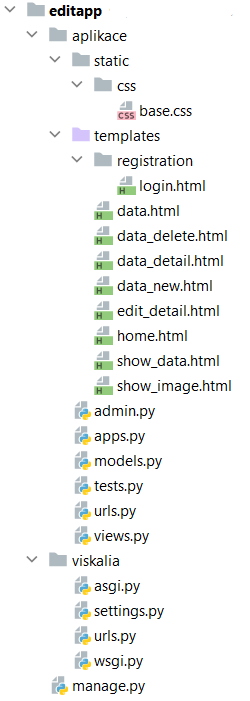
\includegraphics[width=110pt]{./pictures/7-nahled-adresare.PNG}
    \caption[Náhled projektového adresáře]{Náhled projektového adresáře}
	\label{fig:Náhled projektového adresáře}              
\end{figure}

\section{Nastavení jazyka a času}

Dalším nastavením bylo použití našeho středoevropského času a českého
jazyka. Velice jednoduché nastavení, kdy v \emph{settings.py} je po
vytvoření aplikace nastaven jazyk na angličtinu a čas na \zk{UTC}. Pro
změnu se tedy přepíše LANGUAGE\_CODE = 'en-us' na
LANGUAGE\_CODE = 'cs' a TIME\_ZONE = 'UTC' na
TIME\_ZONE = 'CET'.

\newpage

\section{Administrátorské prostředí}

Po vytvoření základní uživatelské aplikace a úvahách o její funkci jsme dospěli k rozhodnutí, že nám bude stačit administrátorské rozhraní, ve kterém se budou provádět modifikace podle daných požadavků.
Při jeho tvorbě a modifikaci byla jako podklad použita oficiální dokumentace Django (\emph{docs.djangoproject.com}) a \cite{django-admin-book} Administrátorské prostředí se upravuje v adresáři aplikace v souboru \emph{admin.py} a lze se do něj dostat zadáním \emph{/admin} za \zk{URL} adresu webové stránky. Začalo se tedy importem a zaregistrováním modelů do rozhraní a vytvořením jejich tříd. Pro model CvutImages se nejprve vytvořila třída PostImageAdmin, ve které je použit StackedInline model. Ten se používá pro vnořené třídy, tedy pokud je chceme zobrazit na jedné stránce společně s jinou třídou. V tomto případě tedy chceme zobrazit obrázky, které přísluší jednotlivým záznamům v třídě Cvut. @admin.register slouží k zobrazení třídy v administrátorském rozhraní, podmíněno vytvořením třídy tohoto modelu, ve které se poté provádí modifikace zobrazení. Ta je zde rozšířena o třídu PostImageAdmin. Dále je zaregistrován model CvutImages a vytvořena jeho třída pro jeho zobrazení.

\begin{figure}[H] \centering
    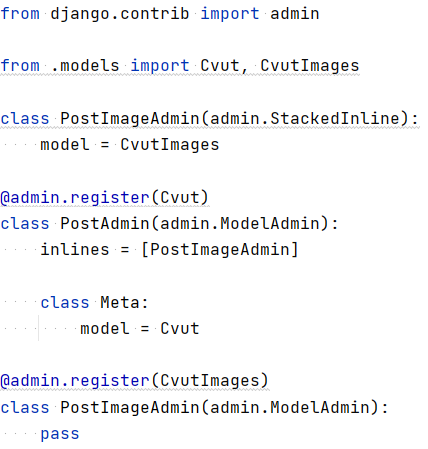
\includegraphics[width=230pt]{./pictures/12-admin-reg.PNG}
    \caption[Registrace modelů v admin.py]{Registrace modelů v admin.py}
	\label{fig:Registrace modelů v admin.py}              
\end{figure}

\newpage

\section{Oprávnění k objektům}
\label{pop}
Dalším úkolem bylo zajištění oprávnění k objektům (per object permissions), tedy že uživatel nebude moci editovat celou tabulku, ale jen objekty, ke kterým bude mít udělená práva. Tuto možnost zajišťuje přídavný balíček \emph{django-guardian}, který ovšem po jeho instalaci a implementaci nefungoval správně a i po nastavení práv uživatel nemohl daný objekt editovat. Vymyslel se tedy systém za použití autentifikačního systému, kdy se do tabulky Cvut přidá nová proměnná Managers, ve které se budou moci vybírat registrovaní uživatelé. Tato proměnná vytváří v databázi novou tabulku, která obsahuje \zk{ID}, \zk{ID} uživatele a \zk{ID} objektu v tabulce. Ve vytvořených třídách v \emph{admin.py} je poté možnost pomocí funkcí has\_view\_permission(), has\_add\_permission(), has\_change\_permission() a has\_delete\_permission() mo\-difikovat práva k tabulkám. Zde se tedy změnilo nastavení funkcí tak, aby tabulky mohl editovat superuživatel, uživatel, který má udělená práva editovat celou tabulku nebo uživatel, který je přidaný v tabulce Managers. 

\begin{figure}[H] \centering
    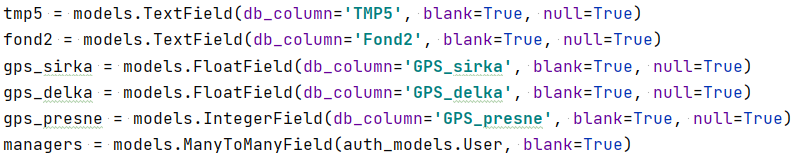
\includegraphics[width=330pt]{./pictures/11-managers-model.PNG}
    \caption[Vytvoření managers v modelu aplikace]{Vytvoření managers v modelu aplikace}
	\label{fig:Vytvoření managers v modelu aplikace}              
\end{figure}

\begin{figure}[H] \centering
    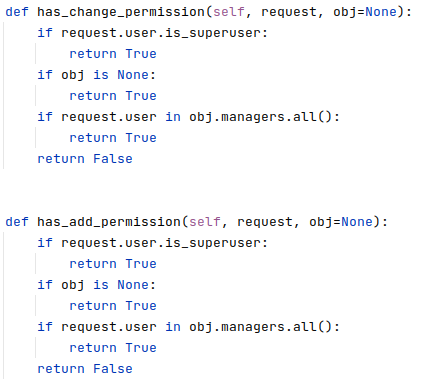
\includegraphics[width=250pt]{./pictures/14-object-permissions.PNG}
    \caption[Úprava práv k objektům]{Úprava práv k objektům}
	\label{fig:Úprava práv k objektům}              
\end{figure}


\section{Nastavení zobrazení dat a jejich vyhledávání}

Django disponuje řadou funkcí pro nastavení zobrazení dat v administrátorském prostředí. Nejprve se nastavovalo zobrazení dat na stránce tabulky. Zde se měly zobrazovat pouze základní informace o objektu jako je \zk{ID}, fond, okres, obec. To se nastavuje pomocí proměnné \emph{list\_display} a \emph{list\_display\_links} slouží pro určení položek, díky kterým se po kliknutí dostanete na stránku obsahující informace o daném objektu. Na této stránce se zobrazují všechny určené položky definované v listu \emph{fields}. Dále byly nastaveny filtry pomocí \emph{list\_filer} a vyhledávání \emph{search\_fields}. 

\begin{figure}[H] \centering
    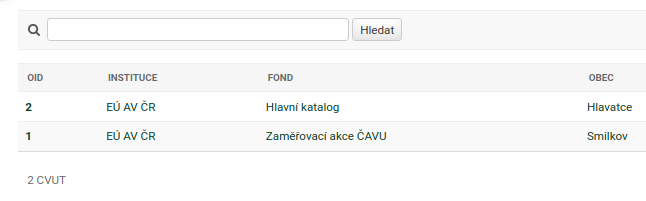
\includegraphics[width=400pt]{./pictures/21-zobrazeni-dat.PNG}
    \caption[Zobrazení dat a vyhledávání]{Zobrazení dat a vyhledávání}
	\label{fig:Zobrazení dat a vyhledávání}              
\end{figure}

\begin{figure}[H] \centering
    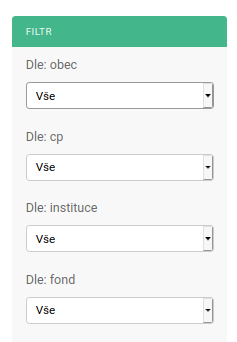
\includegraphics[width=140pt]{./pictures/22-filtry.PNG}
    \caption[Vyhledávání podle filtrů]{Vyhledávání podle filtrů}
	\label{fig:Vyhledávání podle filtrů}              
\end{figure}

\newpage

\section{Použití balíčku admin\_interface}

Při hledání jednoduché a efektivní cesty pro úpravu administrátorského prostření byl vybrán balíček \emph{admin\_interface}. Umožňuje superuživateli po přihlášení do aplikace možnost editovat vizuální stránku aplikace jako změnu loga, nadpisu nebo barvy textu a pozadí. Instalace balíčku viz kapitola 2.1.4 Django - balíčky. Pro správnou funkci je nutno INSTALLED\_APPS v \emph{settings.py} rozšířit nejen o \emph{admin\_interface} ale také o \emph{colorfield}.



\section{Tvorba databáze}
\label{tvorba-database}
Po vytvoření základních funkcionalit aplikace byla projektovému týmu zprostředkována databáze s daty, která se mají zobrazovat. Forma poskytnutých dat byla specifikována v kapitole [\ref{centralni-db}]. Django nedisponuje jednoduchým řešením, jak redukovat duplicitní záznamy a přiřadit jednotlivé obrázky k jednomu záznamu. Úkolem projektového týmu tedy bylo vymyslet řešení, které by tento problém odstranilo. Jako nejlepší řešení se ukázalo z původní tabulky (Base\_Data) exportovat data se sloupci, které příslušely k jednotlivým objektům a vložit je do nové tabulky. Tímto vznikla samostatná tabulka všech objektů (Cvut). Dále se z původní tabulky vybraly sloupce, kde byly umístěny informace o uložených fotografiích a byly opět vloženy do samostatné tabulky (Base\_Images). Tato tabulka byla pomocí cizího klíče propojena s tabulkou Cvut, kde se fotografie odkazovaly na jednotlivé objekty. Data se tedy dostala do normalizované podoby podle třetího stupně.

\begin{figure}[H] \centering
    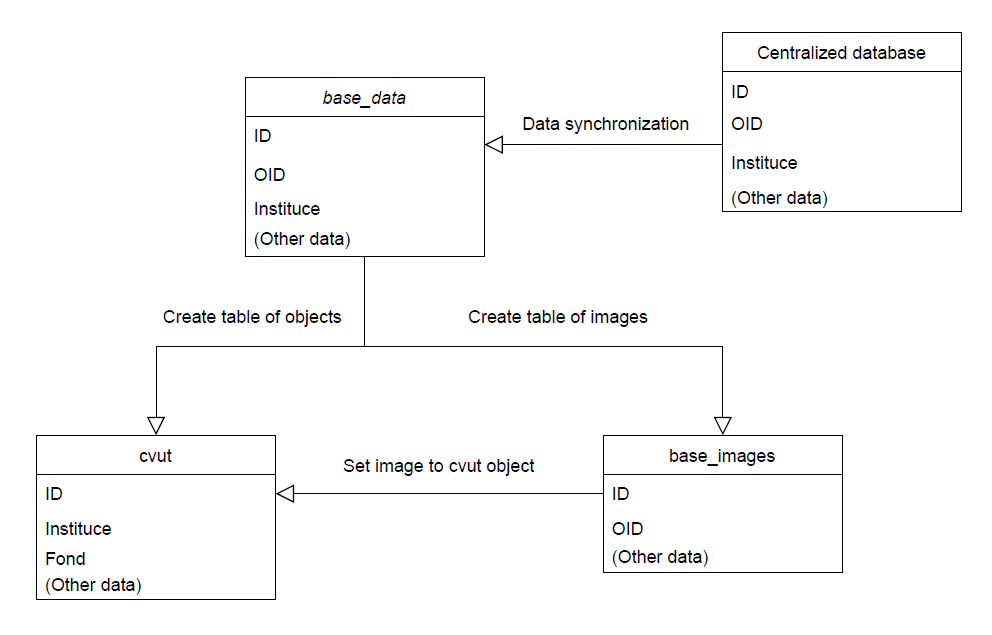
\includegraphics[width=270pt]{./pictures/18-db-diagram-1.PNG}
    \caption[Struktura normalizované databáze]{Struktura normalizované databáze}
	\label{fig:Struktura noramlizované databáze}              
\end{figure}

\section{Doplnění výběrové databáze}

Tato databáze už obsahuje data z centrální databáze, které se pomocí
skriptu upra\-vily dle kapitoly [\ref{tvorba-database}]. Po konzultaci
projektového týmu se dospělo k závěru, že se k jednotlivým objektům
budou přidávat nejen obrázkové soubory, ale také modely a jiné
dokumenty. Vytvořila se tedy tabulka CvutFiles, která odpovídala
tabulce z kapitoly [\ref{Přidání obrázků}], ovšem s tím rozdílem že místo
ImageFile byl použit FileField a byla doplněna o textové informace
jako popis nebo typ dokumenty. Tabulka Cvut se opět rozšířila o
sloupec Managers viz kapitola [\ref{pop}].

\begin{figure}[H] \centering
    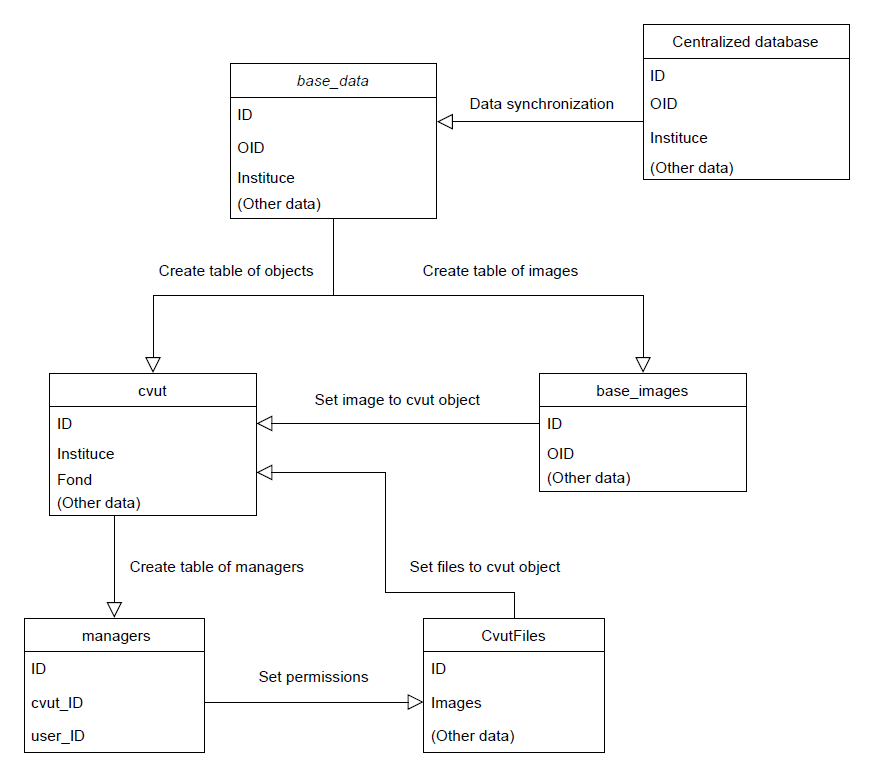
\includegraphics[width=400pt]{./pictures/23-db-diagram-2.PNG}
    \caption[Struktura výběrové databáze]{Struktura výněrové databáze}
	\label{fig:Struktura výběrové databáze}              
\end{figure}

\newpage

\section{Automatizace nasazení aplikace a databáze}


Úkolem projekčního týmu bylo vytvořit prostředí pro jednotný vývoj
aplikace. Do tohoto prostředí bylo ovšem potřeba zahrnout jak aplikaci,
tak databázi, ke které se aplikace připojuje. Základním souborem pro
tvorbu obrazů je \emph{docker-compose.yml}. Ten definuje základní
nastavení pro vytváření tří obrazů, ze kterých se budou spouštět
jednotlivé kontejnery. Prvním obrazem je db, ze kterého vzniká
kontejner, ve kterém běží vytvořená databáze MariaDB. Druhým obrazem
je phpmyadmin, který se nesestavuje lokálně, ale je stažen z
\emph{hub.docker.com}. Třetí obraz je nazván editapp a vytváří kontejner, ve
kterém běží vyvíjená webová aplikace. U každého obrazu je zde potom
definováno, z jakých souborů se obraz vytvoří, název kontejneru, port,
na kterém daný kontejner poběží a další nastavení, potřebná pro
zajištění správného chodu kontejnerů.

Vytvoření obrazu db je definováno z adresáře \emph{mariadb}, kde v
souboru \emph{Dockerfile} je přesně popsáno jeho sestavení. Jako první
je zde definováno sestavení databáze mariadb. Dále je zde doinstalován
soubor \emph{requirements.txt}, který obsahuje potřebná
rozšíření. Dalším souborem \emph{init.py} se vytváří základní tabulka
Base\_Data, která se striktně vytváří dle aktuální verze centrální
databáze a neimituje její změny. S touto tabulkou se pomocí skriptu
\emph{sync-db.py} synchronizují data z centrální databáze, a nakonec
se pomocí \emph{permissions.sql} vytvoří superuživatel, a nastaví se
práva v databázi.

Vytvoření obrazu s webovou aplikace je nastaveno na adresář
\emph{ediatapp}, a je definován pomocí \emph{Dockerfile}. Definice
image je nastavena na Python 3.9, ve kterém také běží Django. Dále se
opět musí doinstalovat potřebná rozšíření, zapsaná v
\emph{requirements.txt} a spustí se skript \emph{startup.sh}. Tímto
skriptem se databáze doplňuje o další tabulky a jejich
objekty. Nejprve se zde provede {\tt python manage.py inspectdb}, kterým se vytvoří
\emph{models.py} s tabulkou Base\_Data. Vytvořený model je rozšířen o
tabulky Cvut, CvutFiles a Base\_Images a migrací je převeden do
databáze. Toto je z důvodů autentifikačního systému, kdy Managers,
které jsou v modelu zapsány v tabulce Cvut vytváří v databázi vlastní
tabulku. Pokud by se vytvořila tabulka Managers v databázi a pomocí
 {\tt python manage.py inspectdb} by se převedla do modelu, vytvořila by se tam jako
samostatná tabulka a nesplňovala by požadovanou
funkcionalitu. Vytvořené tabulky Cvut a Base\_Images se pomocí \zk{SQL}
příkazů v \emph{cvut.sql} doplní o data z tabulky Base\_Data. Obrázky
na které se odkazují jsou momentálně předpřipravené a uložené na
serveru \emph{geo102.fsv.cvut.cz}, odkud se stáhnou a uloží do složky
\emph{media}. Nakonec se aplikace spustí příkazem  {\tt python manage.py runserver}.

\begin{figure}[H] \centering
    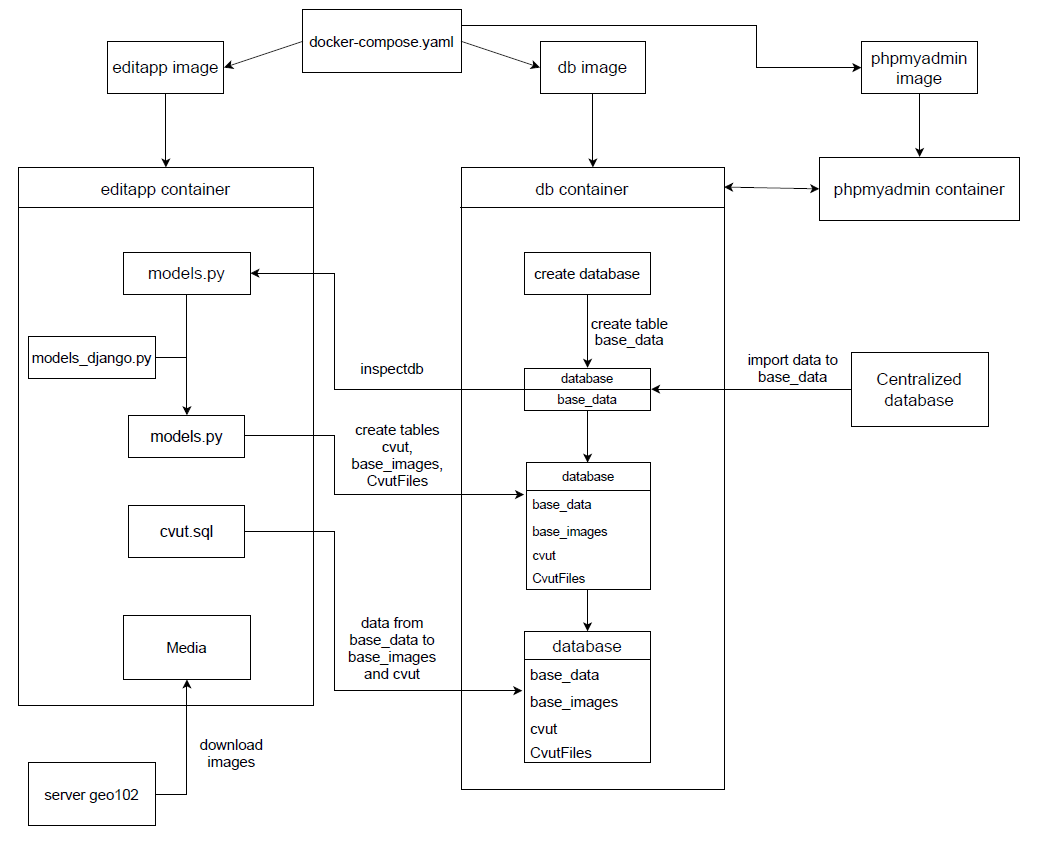
\includegraphics[width=400pt]{./pictures/diagram-docker.PNG}
    \caption[Postup tvorby aplikace a databáze]{Postup tvorby aplikace a databáze}
	\label{fig:Postup tvorby aplikace a databáze}              
\end{figure}


\newpage

\section{Úprava admin prostředí}

S přidáním nové tabulky a nových proměnných bylo potřeba upravit
zobrazení v administrátorském prostředí. Data z centrální databáze
uživatelé nebudou moci přidávat, editovat ani mazat. U tabulek
Cvut a Base\_Images byly proto tyto možnosti úplně odstraněny a tabulka
Base\_Images byla nastavena, aby se její fotografie, které jsou v ní
uložené, zobrazovaly u jednotlivých objektů. U tabulky CvutFiles byla
nastavena možnost přidávání, editace nebo mazání souborů
administrátorům a uživatelům s oprávněním k danému objektu. Bylo také
upraveno zobrazení dat jak v hlavní nabídce, tak na stránce
zobrazující informace o daném objektu. U obrázků byl také vytvořen
jejich náhled v administrátorském prostředí s možností jejich
zvětšení.

\begin{figure}[H] \centering
    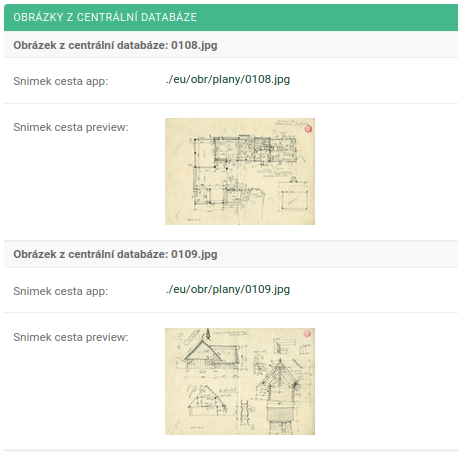
\includegraphics[width=220pt]{./pictures/24-nahled-obrazku.PNG}
    \caption[Zobrazení fotografié v administrátorském prostředí]{Zobrazení fotografié v administrátorském prostředí}
	\label{fig:Zobrazení fotografié v administrátorském prostředí}              
\end{figure}

\begin{figure}[H] \centering
    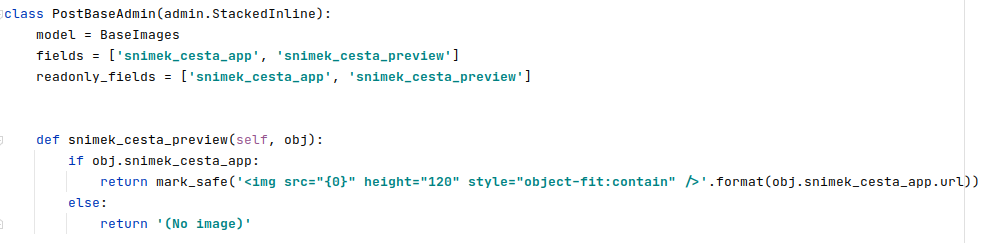
\includegraphics[width=450pt]{./pictures/25-vytvoreni-nahledu.PNG}
    \caption[Vytvoření náhledu v admin.py]{Vytvoření náhledu v admin.py}
	\label{fig:Vytvoření náhledu v admin.py}              
\end{figure}





































